\section{Formål}
I dette domæne analyseres teknologiens virkningsgrad ud fra et klinisk synspunkt. For at kunne danne et vurderingsgrundlag for, hvorvidt QST skal implementeres som supplement til klinikerens vurdering, er det nødvendigt at undersøge teknologiens effektivitet og egentlige effekt.\\
For at kunne vurdere virkningsgraden af QST er det nødvendigt at undersøge de gavnlige og ikke-gavnlige effekter ved brug af teknologien. Denne effektvurdering skal danne grundlag for forståelsen af, hvordan QST kan fungere som supplement til klinikerens beslutning. Ligeledes vil effekten af teknologien sammenholdes med de eventuelle sikkerhedsmæssige risici. Dette skal samlet bidrage til beslutningen om hvorvidt udbyttet af QST er tilstrækkelig i forhold til de sikkerhedsmæssige risici, og i hvilken grad QST kan benyttes som supplement. \\
Ifølge analysen omhandlende klinikerens vurdering, er denne mangelfuld i forhold til identificering af patienter med kroniske postoperative smerter. Beslutningen bygger ikke på tilstrækkelig viden, hvoraf det er relevant at vurdere nøjagtigheden af QST. Nøjagtigheden af resultaterne fra QST skal undersøges, med henblik på at belyse hvorvidt patienter som udvikler kroniske postoperative smerter kan identificeres mere præcist ved anvendelse af QST end uden QST. Derudover vil det også være relevant at undersøge, hvor stor en andel af patienter uden kroniske postoperative smerter teknologien kan identificere. Da patienterne med kroniske postoperative smerter bør kunne identificeres præoperativt med QST som supplement, er det relevant at undersøge hvordan QST-resultaterne for patienter uden kroniske postoperative smerter og en patient med kroniske postoperative smerter adskiller sig fra hinanden. Repeterbarheden for QST undersøges ydermere for at kunne vurdere dens egnethed som et pålideligt supplement til klinikerens beslutning.

\section{HTA spørgsmål}
Statistisk effekt:
\begin{itemize}
	\item \textit{Hvordan opfylder QST-undersøgelserne statistiske parametre som kan anvendes til bestemmelse af klinisk effekt?} %D0001, 
\end{itemize}
Nøjagtighed:
\begin{itemize}
	\item \textit{Hvordan adskiller de præoperative QST-resultater sig fra patienter med kroniske postoperative smerter og patienter uden kroniske postoperative smerter?} %B0018, B0008, B0009, B0010d
	\item \textit{Hvorvidt er undersøgelser med QST repeterbare?} 
\end{itemize}
%\subsection{Metode \citep{HTAcore}}
%For at besvare analysespørgsmålene, foretages en systematisk litteratursøgning i relevante databaser som PubMed, Medline, Cochrane library med mere. Grundlæggende vil vurderingen af relevante artikler vurderes i forhold til evidenshirakiret (se afsnit ref{xx} ). Dette betyder at som udgangspunkt vil meta-studier og randomiserede studier være at foretrække. I forhold til at opnå indsigt i sundhedsfordele og ulemper der er relateret til QST vil studier hvori der indgår information om mortalitet, morbiditet og quality of life blive taget i betragtning. For at opnå viden om nøjagtigheden af QST, vil studier hvori teknologiens sensitivitet og specificitet dokumenteres blive taget i betragtning. Ved vurdering af virkningsgradens normale forhold, kan det blive nødvendigt at undersøge om virkningsgraden kan extrapoleres fra virkning under optimale forhold til normale forhold.

\section{Metode}
For at opnå viden om den kliniske effekt af QST-undersøgelserne, vil der medtages studier hvori QST-parametrenes statistiske signifikans og styrke undersøges. Ligeledes er studier der undersøger nøjagtigheden af QST-parametrene anvendt som et inklusionskriterie. Studier er fundet gennem litteratursøgningen som er beskrevet i \secref{sec_lit}, hvor søgetermer er tilpasset hvert HTA-spørgsmål (se \appref{app_EFFsog} for de specifikke søgetermer). Til besvarelse af de opstillede HTA-spørgsmål er publicerede studier og lærebøger anvendt. 
Studiernes resultater for den statistiske forskel vil blive sammenlignet, sådan effekten kan bedømmes og det kan vurderes hvorvidt QST kan bidrage til klinikerens beslutning. Dette gøres ved vurdering af styrken i QST resultaterne der skal bedømme hvorvidt en patient vil, eller ikke vil, udvikle kroniske postoperative smerter. Herunder vil nøjagtighed og repeterbarhed vurderes for at bedømme om QST kan fungere som et pålideligt supplement, ved vurdering af signifikansen af resultater fra studierne.

\section{Statistisk effekt}
\textit{I dette afsnit undersøges de statistiske parametre som kan anvendes til at undersøge QST-undersøgelsernes kliniske effekt. Først undersøges den statistiske signifikante forskel flere studier har fundet og hvilke konklusioner der kan drages ud fra denne forskel. Herudover vurderes styrken for den signifikante forskel, for at undersøge hvor megen betydning resultaterne for QST-undersøgelserne har for detekteringen for udviklingen af kroniske postoperative smerter. Ligeledes undersøges det hvilken betydning en undersøgelses senstivitet og specificitet vil have for QST-undersøgelsernes egnethed som supplement til en klinikers vurderingsgrundlag.}

\subsection{QST-undersøgelsernens statistiske styrke}
Det er af flere studier fundet, at PPT, TSP og CPM kan være prædiktive for udviklingen af kroniske postoperative smerter. \citep{Wylde2016c} \citep{Petersen2016} Studierne baserer disse resultater på statiske analyser. For at bestemme hvorvidt der er en statistisk forskel mellem de præoperative QST-resultater for patienter uden kroniske postoperative smerter og præoperative QST-resultater for patienter med kroniske postoperative smerter kan der udregnes en p-værdi. En p-værdi er en betegnelse for sandsynligheden for at opnå et resultat der er det samme eller mere ekstremt end det der er blevet fundet i studiet. Denne definition for p-værdien gælder, hvis det antages at der ingen statistisk signifikant forskel er mellem de to datasæt. En lav p-værdi betyder hermed en lille sandsynlighed for at en funden forskel imellem to datasæt skyldes tilfældige samplingsfejl. En stor p-værdi derimod antyder, en stor sandsynlighed for, at en funden forskel skyldes tilfældige samplingsfejl. Normalt anvendes en p-værdi på 0,05 som skillelinjen, hvor værdier under 0,05 angiver, at der er fundet en statistisk signifikant forskel, mens der ved værdier over 0,05 ikke findes en signifikant forskel. \citep{Zar2010} \\
I et studie af \citer{Petersen2016} blev der fundet en signifikant forskel på postoperativ smertelindring for patienter med faciliteret TSP og mindsket CPM i forhold til patienter med enten faciliteret TSP eller mindsket CPM. Disse forskelle blev i studiet vurderet signifikante på baggrund af p-værdier på henholdsvis 0,023 og 0,007. I modsætning til dette blev der fundet en forskel på postoperativ smertelindring for patienter med faciliteret TSP og mindsket CPM og patienter med normal TSP og CPM, men denne var ikke signifikant. For forskellen mellem disse to grupper var p-værdien 0,087. \citep{Petersen2016} Dette er problematisk, da det antyder, at QST-undersøgelserne ikke signifikant kan skelne mellem patienter med anormale resultater og patienter med normale resultater. \\ %det er slettet at der skal være to resultater
Flere andre studier har ligeledes fundet en signifikant sammenhæng mellem en af de tre QST-parametre og kroniske postoperative smerter. \citep{Wylde2013} \citep{Wright2015} I et studie af \citer{Wright2015} blev det fundet at der var en signifikant forskel på postoperativ smerte for patienter med lave præoperative PPT-værdier i forhold til patienter med højere præoperative PPT-værdier. Her blev der fundet en p-værdi på 0,002 for PPT målt ved albuen. Denne p-værdi angiver, at der er en lille sandsynlighed for at de fundne resultater skyldes en samplingsfejl, hvormed det kan indikeres at PPT kan anvendes som indikator for postoperativ smerte mellem 12 og 36 måneder efter operationen. \citep{Wright2015} I et studie af \citer{Petersen2015} blev der fundet en signifikant forskel på patienter med en faciliteret TSP og patienter med normal TSP, i forhold til udviklingen af postoperative kroniske smerter. Denne signifikante forskel blev vurderet på baggrund af en p-værdi på 0,009, hvormed sandsynligheden for at den observerede forskel skyldes samplingsfejl er på 0,9\%. I studiet af \citer{Petersen2015} blev CPM ligeledes undersøgt, men der blev for denne QST-parameter ikke fundet nogen signifikant forskel. \\
Det kan udfra ovenstående udledes at flere studier har fundet, at det ved fænotypebestemmelse af patienter ud fra både PPT, TSP og CPM er muligt at finde en signifikant forskel mellem fænotyper i forhold til kroniske postoperative smerter. Det er dog problematisk at nogle studier ikke finder en signifikant forskel mellem fænotyperne. \citep{Leary2016} Herudfra er det relevant at undersøge hvor stærk sammenhængen er mellem de præoperative QST-resultater og kroniske postoperative smerter.

\subsubsection{Korrelationsstyrke}
Den kliniske effekt af QST-undersøgelserne kan undersøges ved analyse af korrelationskoefficienterne (R-værdierne) for PPT, TSP og CPM. En korrelationskoefficient kan anvendes til at bestemme styrken af sammenhængen mellem to datasæt. Dermed undersøges det i hvilket omfang værdierne fra det ene af datasættene er afhængig af værdierne fra det andet datasæt. \citep{Zar2010} \\
R-værdien er et enhedsløst tal, der kan ligge i intervallet mellem -1 og 1. Sammenhængen mellem to datasæt med en R-værdi på -1 har negativ korrelation, hvor værdierne for det ene datasæt stiger, mens værdierne for det andet datasæt falder. Hvis R-værdien for en sammenhæng er 1 vil datasættene være positivt korreleret, hvilket betyder værdierne for det ene datasæt stiger når værdierne for det andet datasæt stiger. Hvis der ingen korrelation er mellem to datasæt vil R-værdien være 0. \citep{Zar2010} Disse korrelationer er illustreret på \figref{fig:r_vaerdi}

\begin{figure}[H]
\centering
\includegraphics[scale=.8]{figures/dHTAanalyse/r_vaerdi}
\caption{Figuren illustrerer forskellige muligheder for korrelation mellem to datasæt. For disse grafer er Y det afhængige datasæt, mens X er uafhængig. Graf (a) illustrerer en positiv korrelation mellem X og Y, hvormed R-værdien er lig 1. På graf (b) vises negativ korrelation mellem X og Y, med en R-værdi på -1. For graf (c) og (d) er R-værdien 0, og der er dermed ingen korrelation mellem X og Y. \textit{Fra \citer{Zar2010}}}\label{fig:r_vaerdi}
\end{figure}

Som det ses ud fra \figref{fig:r_vaerdi} er der større korrelation mellem to datasæt jo tættere på 1 |R| kommer. Hermed bestræber studier, der finder en statistisk sammenhæng mellem to datasæt, sig på, at den numeriske værdi af R for sammenhængen er så tæt på 1 som muligt. Styrken af sammenhængen mellem to datasæt ud fra R-værdien kan ses i \tabref{tab:styrke_r}. \\

\begin{table}[H]
\centering
\begin{tabular}{cc}
\rowcolor[HTML]{C0C0C0} 
R-værdi {[}numerisk{]} & Betydning  \\ \hline
0,9 til 1              & Meget høj korrelation              \\
0,7 til 0,9            & Høj korrelation                    \\
0,5 til 0,7            & Moderat korrelation                \\
0,3 til 0,5            & Lav korrelation                    \\
0 til 0,3              & Ingen korrelation                  \\ \hline
\end{tabular}
\caption{Tabellen viser betydningen af forskellige R-værdier. R-værdierne er angivet som numeriske værdier, hvormed betydningen af værdierne gælder for både positive og negative korrelationer. \textit{Tabellen er modificereret fra \citer{Mukaka2012}}}
\label{tab:styrke_r}
\end{table}

Flere studier som har fundet en statistisk signifikant sammenhæng mellem en af det tre QST-parametre, har ligeledes undersøgt R-værdien for denne sammenhæng. For et studie af \citer{Wylde2013} blev der fundet en statistisk signifikant sammenhæng mellem præoperative PPT-resultater og udviklingen af kroniske postoperative smerter med en p-værdi på 0,008. Korrelationskoefficienten for denne sammenhæng blev fundet til 0,37. Hermed er sammenhængen mellem præoperative PPT-resultater og kroniske postoperative smerter lav, og næsten i en størrelsesorden hvor der ingen korrelation er (jævnfør \tabref{tab:styrke_r}). Denne lave R-værdi er en tendens der er generel for studier, der har fundet en statistisk signifikant sammenhæng mellem en af de tre QST parametre og kroniske postoperative smerter. Eksempelvis er R-værdien for studiet af \citer{Petersen2016}, hvor der findes en sammenhæng mellem præoperativ PPT og postoperativ smertelindring, på -0,216. Udfra \tabref{tab:styrke_r} indikerer denne R-værdi at der ikke er nogen korrelation imellem de to datasæt. Ligeledes er R-værdien fra et studie af \citer{Petersen2015} for sammenhængen mellem TSP og postoperativ kronisk smerte på 0,24. Heller ikke denne R-værdi viser en korrelation. \\
Det at alle af de undersøgte studier har vist lav til ingen korrelation (0 til 0,5), antyder at den individuelle linære sammenhæng mellem de tre QST-parametre og kroniske postoperative smerter er dårlig. Det er i studiet af \citer{Petersen2016} ikke undersøgt korrelationen mellem faciliteret TSP og mindsket CPM sammen og postoperative kroniske smerter, men dette vil kunne gøres ved anvendelse af en mutibel regressionsanlyse. \citep{Zar2010} Hermed vil det være muligt at undersøge om styrken af den linære sammenhæng er stærkere for TSP og CPM samlet end individuelt.

\subsubsection{Sensitivitet og specificitet}
For at en kliniker vil kunne anvende QST-parametrene til at fænotypebestemmme patienter med knæartrose, er det nødvendigt for klinikeren at vide hvor specifik og sensitiv QST-undersøgelserne er. Specificitet og sensitivitet angiver hvor god en undersøgelse er til at finde sande negative og sande positive patienter. Fremadrettet betegnes positive resultater som resultater der antyder central sensibilisering. Dette vil sige at et positivt resultat for PPT er en lav PPT-værdi, mens det for TSP er en høj TSP-værdi og for CPM er en lav CPM-værdi \citep{Petersen2016}. Hermed vil en patient som har et positivt resultat af undersøgelserne være centralt sensibiliseret. \\
Resultater fra en undersøgelse kan opdeles i fire kategorier; sande positive (SP), falske positive (FP), sande negative (SN) og falske negative (FN). Disse fire resultater er illustreret i \tabref{tab:pos_neg}.

\begin{table}[]
\centering
\begin{tabular}{llcc}
\rowcolor[HTML]{C0C0C0} 
\cellcolor[HTML]{C0C0C0}                                 &         & \multicolumn{2}{c}{\cellcolor[HTML]{C0C0C0}Sygdom}        \\ \cline{2-4} 
\cellcolor[HTML]{C0C0C0}                                 &         & \multicolumn{1}{l}{Positiv} & \multicolumn{1}{l}{Negativ} \\
\cellcolor[HTML]{C0C0C0}                                 & Positiv & Sand positiv                & Falsk positiv               \\
\multirow{-4}{*}{\cellcolor[HTML]{C0C0C0}Testresultater} & Negativ & Falsk negativ               & Sand negativ               
\end{tabular}
\caption{Tabellen viser de fire mulige resultater fra en undersøgelse. \textit{Modificeret fra \citer{Parikh2008}} }
\label{tab:pos_neg}
\end{table}

Som det ses ud fra \tabref{tab:pos_neg} kan undersøgelser vise både falsk positive og falsk negative resultater. Disse falske resultater er problematiske, idet resultaterne betyder patienten risikerer kan få den forkerte behandling \citep{Lalkhen2008}. For knæartrosepatienter vil falsk positive resultater betyde at patienten ikke vil blive tilbudt en TKA-operation, selvom denne ikke har central sensibilisering. Ligeledes vil falsk negative resultater betyde at en patient med central sensibilisering vil få en TKA-operation, hvorefter denne patient har betydeligt større risiko for at udvikle kroniske smerter end andre patienter. En undersøgelses sensitivitet og specificitet kan anvendes til at undersøge risikoen for falske resultater. \\
Den matematiske definition af sensitivitet er: \\
\begin{equation}
Sensitvitet=\frac{SP}{SP+FN}
\end{equation}
Herudfra kan det ses at sensitiviteten af en undersøgelse vil stige når antallet af falske negative resultater falder. En undersøgelse med en sensitivitet på 100\% vil korrekt identificere alle patienter med sygdommen. Hvis undersøgelsen har en sensitivitet på mindre end 100\% vil en del af de patienter som har sygdommen, have falsk negative resultater og hermed blive fejldiagnosticeret. Sensitivitet er dermed et udtryk for hvor stor en andel af patienterne med en sygdom undersøgelsen er i stand til at detektere. \citep{Lalkhen2008} \\
Specificitet er det modsatte af sensitivitet, hvilket vil sige en undersøgelses specificitet er et udtryk for hvor mange patienter som ikke har sygdommen undersøgelsen korrekt vil være i stand til at identificere \citep{Lalkhen2008}. Den matematiske definition på specificitet er: \\
\begin{equation}
Specificitet=\frac{SN}{SN+FP}
\end{equation}
Dette betyder at en undersøgelses specificitet stiger når antallet af falske positive resultater falder. \citep{Lalkhen2008} \\
Ideelt set vil en undersøgelse have både en sensitivitet og specificitet på 100\%, hvormed undersøgelsen altid vil identificere patienter med sygdommen som positive og patienter uden sygdommen som negative. Denne type undersøgelse er i de fleste tilfælde urealistiske, hvormed det kan være nødvendigt at lave et kompromis mellem sensitivitet og specificitet. Dette betyder at en undersøgelse med en høj sensitivitet vil have en lav specificitet, og omvendt for en undersøgelse med en høj specificitet. Om en undersøgelse skal have en høj sensitivitet eller en høj specificitet afhænger af sygdommen der undersøges for, og de etiske konsekvenser for hver af de to falske resultater (dette undersøges nærmere for QST-undersøgelser i \chapref{ETH_chap}). \\
Der er på nuværende tidspunkt ikke publiceret data omkring sensitiviteten og specificiteten for QST-undersøgelserne. \citep{Wylde2013} Disse data er essentielle for om QST-undersøgelserne kan anvendes som supplement til klinikerens vurderingsgrundlag, idet det ud fra sensitiviteten og specificiteten kan vurderes hvor stor vægt klinikeren skal lægge i resultater fra undersøgelserne. På \figref{fig:AUC} illustreres tre muligheder for sensitivitet og specificitet:

\begin{figure}[H]
\centering
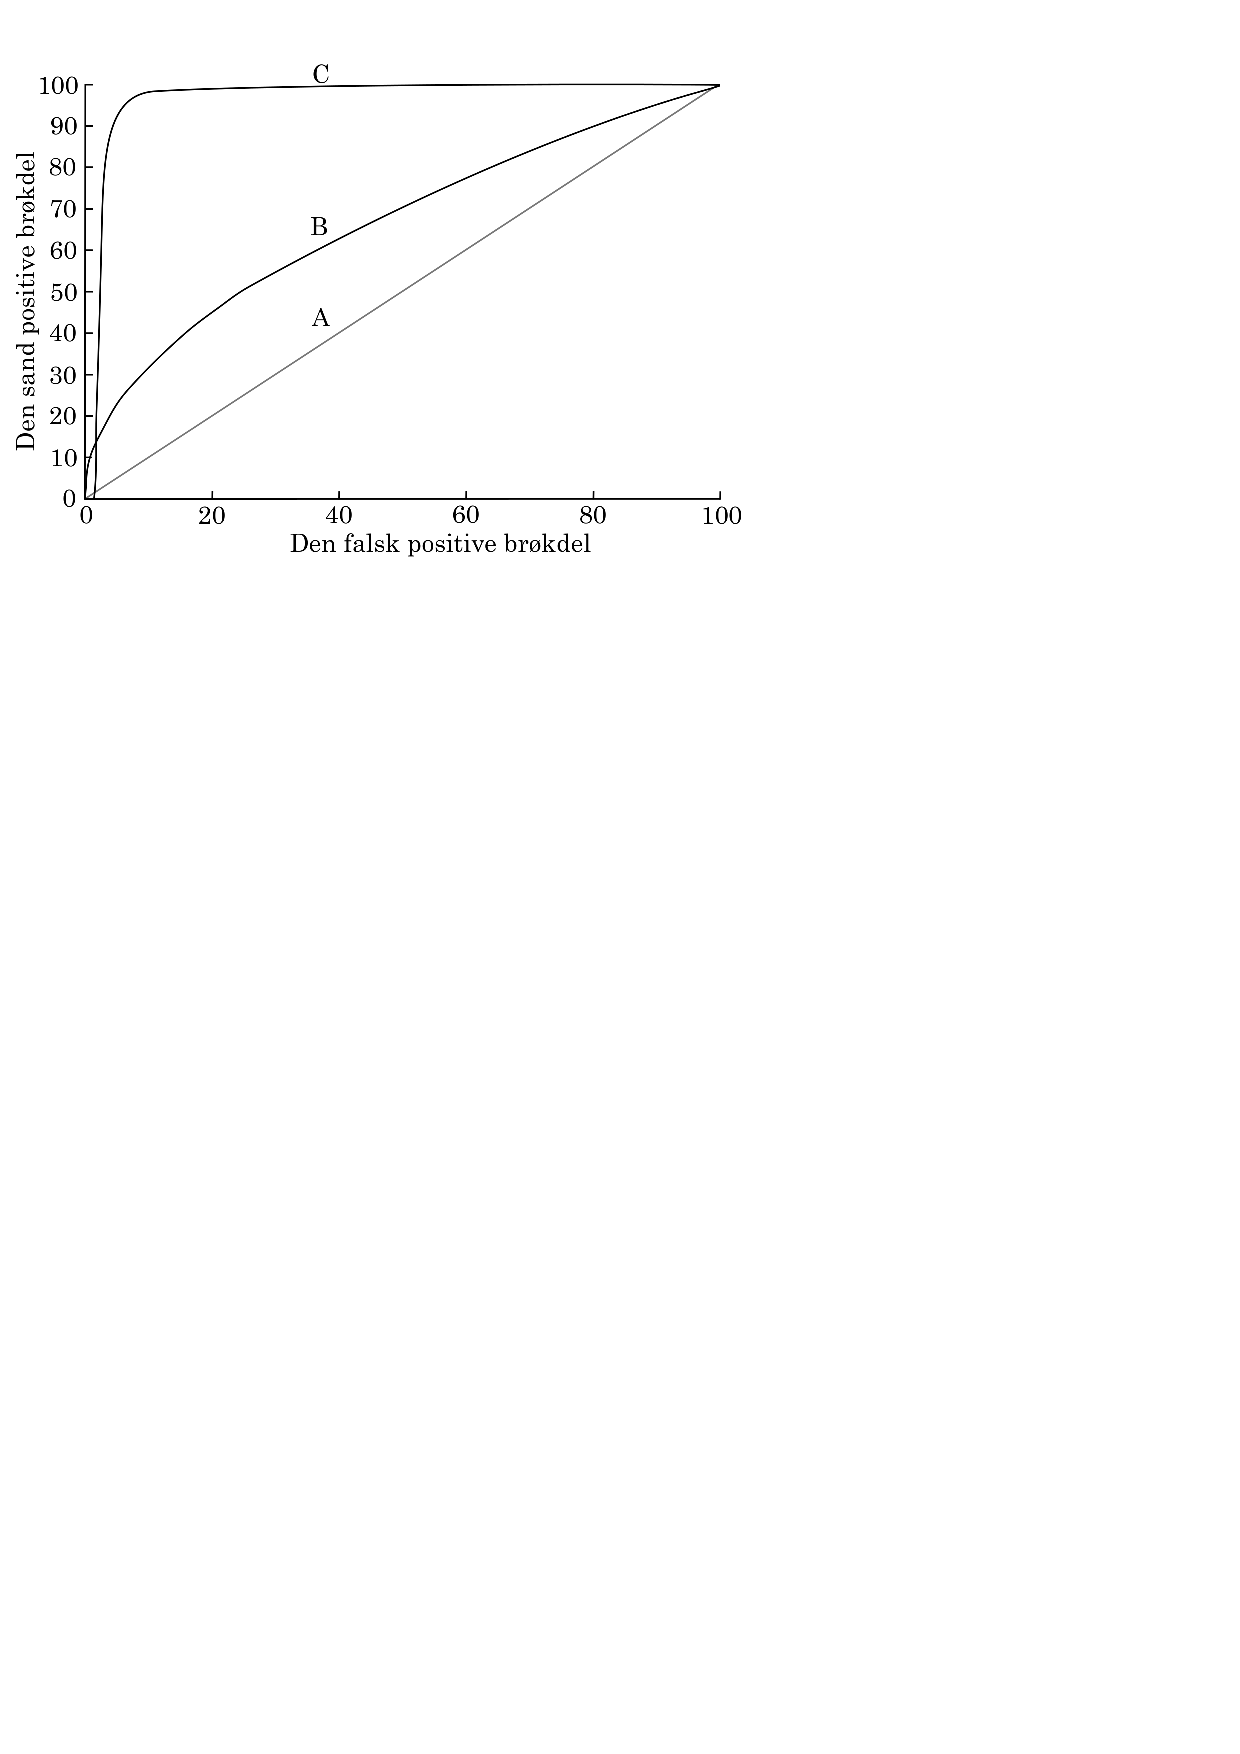
\includegraphics[width=0.7\textwidth]{figures/dHTAanalyse/AUC}
\caption{Figuren illustrerer tre mulige sammenhænge mellem sensitivitet og specificitet, når cut-off værdien for undersøgelsen ændres. Op af y-aksen er den sande positive brøkdel (sensitiviteten) angivet, mens den falske positive brøkdel (100-specificiteten) er hen ad x-aksen. Linje C viser plottet for en ideel undersøgelse, mens linje B viser det typiske plot for en undersøgelse som anvendes normalt i klinisk praksis. Den stiplede linje, A, viser linjen for nul diskrimination. \textit{Fra \citer{Lalkhen2008}}}\label{fig:AUC}
\end{figure}

Den stiplede linje, A, som vises på \figref{fig:AUC}, angiver linjen for nul diskrimination. Dette betyder at undersøgelser hvis plot ligger på denne linje ikke kan skelne mellem sande positive og sande negative, og resultater fra undersøgelsen har 50\% risiko for at være forkerte. Arealerne under kurverne angiver præcisionen for en undersøgelse, hvor en ideel undersøgelse (linje C) har et areal under kurven på 1 mens nul diskriminationslinjen (linje A) har et areal under kurven på 0,5. \\
Udfra dette vil QST-undersøgelserne, før disse kan være anvendelige for en kliniker, skulle have en præcision der er højere end 0,5 og så tæt på 1 som muligt. Hvis QST-undersøgelserne ikke har denne præcision vil disse være svære for klinikeren at anvende, hvormed det er nødvendigt at undersøge sensitivitet og specificitet for undersøgelserne.   

\section{Nøjagtighed}
\textit{I følgende afsnit vil forskellen i QST-resultater undersøges for patienter som udvikler kroniske postoperative smerter, og patiente som ikke gør. Ligeledes vil QST-undersøgelsernes nøjagtighed blive beskrevet, både i forhold til dets resultater, men også i forhold til teknologiens relibilitet. Dette er for at kunne vurdere egentheden af QST-undersøgelserne, som et brugbart supplement.}

\subsection{Patientgruppering på baggrund af QST-resultater}
Det forsøges at skabe en præoperativ fænotypebestemmelse, som indikerer hvorvidt en patient er disponeret for at udvikle kroniske postoperative smerter. Som nævnt i \chapref{TEC_chap} er der en indikation på at nedsat PPT, forhøjet TSP og nedsat CPM er de diagnostisk relevante QST-parametre, til at kunne skabe den omtalte smerteprofil. \\
Studiet af \citer{Suokas2012} har undersøgt forskellige studiers PPT-resultater for både raske kontrolpersoner og personer som lider af knæartrose. Studierne undersøgt af \citer{Suokas2012} bestemte PPT ud fra forskellige anatomiske placeringer, eksempelvis, på det påvirkede knæ, under det påvirkede knæ samt væk fra det påvirkede knæ. For patienter som led af knæartrose, var henholdsvis den laveste og højeste gennemsnitlige PPT-værdi på 177 kPa ($\pm$ 98) og 512 kPa ($\pm$ 221), hvilket var lavere end hos de raske kontrolpersoner. De raske kontrolpersoner opnåede gennemsnitlige PPT-værdier på imellem 333 kPa ($\pm$ 82) og 1098 kPa ($\pm$ 199). \citep{Suokas2012} Denne indikation på, at personer med knæartrose har en lavere PPT-værdi end raske personer, er ligeledes vist i studiet af \citer{Wylde2013}, som testede PPT på det påvirkede knæ, samt på underarmen. De raske forsøgspersoner opnåede i gennemsnit PPT-resultater på henholdsvis 405 kPa på knæet og 339 kPa på underarmen. Knæartrosepatienterne havde i studiet af \citer{Suokas2012}, lavere PPT-resultater end de raske kontrolpersoner. Den gennemsnitlige PPT-værdi for knæartrosepatienterne var henholdsvis 155 kPa på knæet og 171 kPa på underarmen. \citep{Wylde2013} 

\begin{table}[H]
	\centering
	\resizebox{\textwidth}{!}{%
		\begin{tabular}{ccc}
			\hline
			\rowcolor[HTML]{C0C0C0} 
			Studie               & Kontrol patientgruppe: PPT {[}kPa{]} & Knæartrose patientgruppe: PPT {[}kPa{]} \\ \hline
			\citer{Suokas2012} & 333 ($\pm$ 82) til 1098 ($\pm$ 199)      & 177 ($\pm$ 98) til 512 ($\pm$ 221)          \\
			\citer{Wylde2013}  & 405 (knæ) og 339 (underarmen)        & 155 (knæ) og 171 (underarmen)           \\ \hline
		\end{tabular}
	}
	\caption{I tabellen ses resultaterne vedrørende PPT-målinger på henholdsvis raske person og knæartrsoe patienter. }
	\label{tab:PPT_rask_syg}
\end{table}\vspace{-.25cm}

Resultaterne præsenteret i studierne af \citer{Suokas2012} og \citer{Wylde2013}, som ses i \tabref{tab:PPT_rask_syg}, viser at der imellem raske og knæartrosepatienter er en signifikant forskel på gennemsnitlige PPT-værdier. Der ses heraf en tendens til at knæartrosepatienterne kan modstå mindre tryk førend sensationen af stimulus opfattes som smerte, end raske personer.

QST bliver ligeledes benyttet af \citer{Petersen2015} og \citer{Wright2015}, men til at undersøge forskellen af PPT-resultater knæartrosepatienter imellem. \citer{Wright2015} inddelte patienterne som havde undergået en TKA-operation i grupper; en gruppe med moderat til kraftig smerte mindst 12 måneder efter operationen (Gruppe A) og en gruppe uden smerter mindst 12 måneder efter operationen (Gruppe B). Gruppe A havde gennemsnitligt PPT-værdier på 282 kPa ved knæet og på 314 kPa ved den distale albue. Gruppe B havde gennemsnitligt PPT-værdier på 416 kPa ved knæet og på 454 kPa ved den distale albue. Studiet af \citer{Petersen2015} viste ikke samme grad af spredning i resultaterne mellem grupperne med og uden kronisk postoperativ smerte, men viste samme tendens som \citer{Wright2015} grupperne imellem. Gruppen i studiet af \citer{Petersen2016} med lave kroniske postoperative smerter havde en gennemsnitlig PPT-værdi på henholdsvis 600 $\pm$ 25 kPa ved det påvirkede knæ og 460 $\pm$ 10 kPa på armen. Gruppen med høje kroniske postoperative smerter havde en PPT-værdi på 550 $\pm$ 50 kPa ved det påvirkede knæ og 460 $\pm$ 20 kPa på armen. \citep{Petersen2015}

\begin{table}[H]
	\centering
	\resizebox{\textwidth}{!}{%
		\begin{tabular}{ccc}
			\hline
			\rowcolor[HTML]{C0C0C0} 
			Studie                 & Lav smerte gruppe: PPT {[}kPa{]}     & Høj smerte gruppe: PPT {[}kPa{]}     \\ \hline
			\citer{Wright2015}   & 416 (knæ) og 454 (albue)             & 282 (knæ) og 314 (albue)             \\
			\citer{Petersen2015} & 600 $\pm$ 25 (knæ) og 460 $\pm$ 10 (arm) & 550 $\pm$ 50 (knæ) og 460 $\pm$ 20 (arm) \\ \hline
		\end{tabular}
	}
	\caption{I tabellen ses resultaterne vedrørende PPT-målinger på henholdsvis en gruppering med lave og høje kroniske postoperative smerter.}
	\label{tab:PPT_syg_syg}
\end{table}\vspace{-.25cm}
Resultaterne præsenteret i studierne af \citer{Wright2015} og \citer{Petersen2015}, som ses i \tabref{tab:PPT_syg_syg}, viser at der blandt knæartrosepatienter med forskellig grad af kronisk postoperativ smerter, er en forskel i deres PPT-værdier. På baggrund af resultaterne opnår knæartrosepatienter med høje kroniske postoperative smerter, lavere PPT-resultater, end knæartrosepatienter med lave kroniske postoperative smerter. \citep{Wright2015} \citep{Petersen2015}

I et studie af \citer{Vaegter2016} undersøges forskellige smertemoduleringers egenskaber til at kunne fænotypebestemme patienter i forhold til kroniske smerter. Studiet undersøger påvirkningen af QST-parametrene TSP og CPM, på kroniske smertepatienter. Resultaterne fra studiet viser, at kvindelige patienter med nedsat CPM faldt 11,6\% $\pm$ 19,3\% fra det først målte PPT-resultat, og at mandlige patienter med nedsat CPM faldt 3.6\% $\pm$ 17.1\% fra det først målte PPT-resultat. Studiets resultater vedrørende TSP blev opgivet i en VAS ratio for VAS3 over VAS1. VAS3 bestod af gennemsnittet af ottende og niende stimulirespons og VAS1 bestod af gennemsnittet af første til fjedre stimulirespons. Resultaterne for både de kvindelige og mandelige patienter med faciliteret TSP var en VAS-ratio på 1,7 $\pm$ 0,4. Faciliteret TSP og nedsat CPM er påvist at kunne prædiktere kroniske smerte hos patienter der har gennemgået torakotomi og abdominal kirurgi. \citep{Vaegter2016} \\
Studier af \citer{Petersen2016} og \citer{Petersen2015} er det undersøgt hvordan TSP og CPM har indflydelse på en patients kroniske postoperative smerter. I studiet af \citer{Petersen2016} blev det bekræftet at patienter med faciliteret TSP og nedsat CPM var den patientgruppering med fleste kroniske postoperative smerter. I studiet blev det arbitrært bestemt at faciliteteret TSP var resultater over gennemsnittet, og at nedsat CPM var resultater under gennemsnit. CPM blev i studiet bestemt ved at trække PPT-resultat fra CPM-målingen fra det målte PPT-resultat forud for testen, og var gennemsnitligt 5,40 $\pm$ 1,05 kPa. Grupperingen med nedsat CPM havde gennemsnitligt resultatet -2 $\pm$ 0,5 kPa. TSP blev i studiet bestemt ved at trække VAS2 som værende gennemsnittet af måling [8,..,10] fra VAS1 som værende gennemsnitet af måling [1,..,4] og var 1,55 $\pm$ 0,17. Grupperingen med faciliteret TSP havde gennemsnitligt resultatet 3 $\pm$ 0,5. 

\begin{table}[H]
	\centering
	\resizebox{\textwidth}{!}{%
		\begin{tabular}{ccc}
			\hline
			\rowcolor[HTML]{C0C0C0} 
			Studie                 & Gruppering med nedsat CPM                                                                   & Gruppering med faciliteret TSP \\ \hline
			\citer{Vaegter2016}  & \begin{tabular}[c]{@{}c@{}}-11,6 $\pm$ 19,3 \% (kvinder)\\ -3.6 $\pm$ 17 \% (mænd)\end{tabular} & 1,7 $\pm$ 0,4 (kvinder og mænd)  \\
			\citer{Petersen2016} & -2 $\pm$ 0,5 kPa                                                                              & 3 $\pm$ 0,5                      \\ \hline
		\end{tabular}
	}
	\caption{I tabellen ses resultaterne vedrørende CPM og TSP målinger på gruppering med nedsat CPM og faciliteret TSP.}
	\label{tab:CPM_TSP}
\end{table}

Resultaterne præsenteret i studierne \citer{Vaegter2016} og \citer{Petersen2016}, som ses i \tabref{tab:CPM_TSP}, viser at kroniske smertepatienter har nedsat CPM og faciliteret TSP. Det påvises i studierne at patienter med disse tilstand har signifikant flere kroniske smerter. \citep{Vaegter2016} \citep{Petersen2016}

Ovenstående resultater omhandlende patientgruppering for QST-parametrene PPT, TSP og CPM varerier tydeligt. Det ses af resultaterne at det er muligt ved benyttelse af QST, at se forskel på patienter uden central sensibilisering og patienter med. Det kan yderligere ses på resultaterne at der imellem de forskellige studiers resultater ikke er nogen eksakt konsistens, de viser dog samme tendens. Dette kan være en indikation for forskelligt anvendt udstyr, samt undersøgelsens metode. Herfor skal man udføre QST ens alle gange og med samme udstyr før det giver mening at lave et normativt datasæt. Et normativt datasæt til inddeling af patienter i grupperinger, med tilhørende udførelig metode til undersøgelsen, skal udarbejdes førend patienter kan klassificeres som værende i en anormal tilstand. Ovenstående indikerer, at resultaterne for PPT, TSP og CPM varierer imellem knæartrosepatienter, og at disponerede patienter for kroniske postoperative smerter har lavere PPT, faciliteret TSP og nedsat CPM. 

\subsection{Repeterbarhed for QST}
I et studie af \citer{Nielsen2015} er repeterbarheden for manuelt udførte PPT-undersøgelser blevet undersøgt. De 136 forsøgspersoner, der indgik i studiet, blev undersøgt ved brug af et trykalgometer fra Somedic. Forsøget blev udført på låret (quadriceps) og på overarmen (biceps brachii) i forsøgspersonernes dominante side. Studiet var struktureret i to sessioner med minimum en uges mellemrum. Forsøgets resultater viste, at inter-korrelations koefficienten (ICC) mellem de målte data for de to sessioner var 0,89 for ben og 0,87 arme. Begge disse værdier er i studiet defineret som værende høje, da de overskrider den fastsatte tærskelværdi på 0,75. Analysen af resultaterne viste endvidere en bias både for ben og arme i form af en forskel mellem de beregnede middelværdier for de to sessioner. Det samme studie undersøgte repeterbarheden for PPT-undersøgelser udført med computerstyret cuff-algometri. Til denne undersøgelse blev et cuff-algometer fra Nocitech placeret henholdsvis omkring læggen og overarmen i den non-dominante side. Forsøgspersonerne skulle under forsøget kvantificere deres smerte ved hjælp af en elektronisk VAS-tabel. Når smerten blev uudholdelig skulle forsøgspersonerne selv trykke på en knap, der stoppede trykpåvirkningen i cuff-algometeret, hvorefter forsøget var afsluttet. Resultaterne viste en interkorrelationskoefficient på 0,79 for benet og 0,85 for armen, hvilket igen i dette studie er defineret som høje korrelationer. Ligesom for den manuelle PPT-undersøgelse viste dette forsøg en systemisk fejl mellem de to sessioner, men kun for målingerne på armen.

I et litteraturstudie af \citer{Kennedy2016} blev repeterbarheden for CPM-undersøgelser på forskellige områder af kroppen analyseret. Analysen var baseret på 10 studier, hvoraf fem studier anvendte PPT som teststimuli. Typen af konditionerede stimuli varierede imellem de fem studier. I et studie blev den opfølgende test lavet under samme session som den primære, imens der i tre andre studier blev udført en opfølgende test i løbet af to til 10 dage. I det sidste studie blev der både foretaget en opfølgende test i samme session som den primære og yderligere en opfølgning tre dage senere. \citer{Kennedy2016} opdelte studiernes resultater i henholdsvis repeterbarhed for teststimuli og for konditioneret stimuli. Det fremgår, for forsøgene, hvor den opfølgende test er udført i samme session som den primære, at ICC ligger mellem 0,82 og 0,87 for teststimuli (PPT), hvilket overskrider grænsen for høj korrelation på 0,75. For studierne, der har afholdt to uafhængige sessioner ligger ICC i intervallet fra 0,65 til 0,79 og defineres derfor som værende god til høj. For de konditionerede stimuli, hvor den opfølgende test blev lavet i samme session som den primære, lå ICC mellem 0,60 og 0,94. For studierne, der udførte den opfølgende test i en separat session var ICC i et interval fra 0,61 til 0,82.\\ 
Et studie af \citer{Imai2016} undersøgte ligeledes, hvordan CPM-undersøgelsers repeterbarhed påvirkes ved ændring af test- og konditionerede stimuli. I studiet indgik 26 raske mænd. Hver forsøgsperson gennemgik to identiske sessioner med højst tre ugers mellemrum. Der blev anvendt fire forskellige typer teststimuli, hvoraf de to var baseret på tryk (manuel- og cuff-algometri). Trykket blev påført med et algometer fra Somedic og en manchet fra Nocitech. Både det håndholdte og cuff-algometeret var placeret på underbenet ved forsøgene. Den konditionerede stimuli blev påført kontralateralt for teststimuli og var udgjort af cold pressor threshold (CPT) og cuff-algometeret. I studiet er ICC-værdierne for forsøgene med trykbaseret teststimuli henholdsvis 0,49 og 0,44 for CPT, mens de for cuff-algometri er 0,04 og 0,53.\\ 
I studiet af \citer{Nielsen2015} blev TSP undersøgt i forlængelse af de cuff-baserede tests af PPT og smertetolerance (PTT). Undersøgelsen foregik ved at cuff-algometeret blev pustet op til et tryk svarende til den fundne smertetolerance 10 gange af to sekunders varighed. Resultaterne for studiet viste en ICC på 0,60 for benet og 0,43 for armen. 

Flere studier har undersøgt repeterbarheden for udførelsen af PPT- TSP- og CPM-undersøgelser. På baggrund af resultaterne kan det ses, at der generelt forekommer en høj ICC for PPT-undersøgelser baseret på de definerede tærskelværdier i de respektive studier. For CPM-undersøgelser forekommer der generelt en større variation i resultaterne. ICC-værdierne for TSP fundet af \citer{Nielsen2015} er i intervallet middel til god, men dette resultat kan med fordel underbygges af flere studier. 
%% Skal vi nævne at Cuffen er udviklet af AAU
Det er ligeledes væsentligt for vurderingen af den samlede behandling, hvilke tiltag der er mulige, og hvor stor effekten er af disse, hvis QST kan identificere patienter som har en forhøjet risiko for at udvikle kronisk smerte efter en TKA-operation.

\section{Delkonklusion}
Der foreligger endnu ikke nok viden om QST-undersøgelsernes samlede effekt til at vurdere hvorvidt disse vil kunne anvendes som supplement til en klinikers vurderingsgrundlag. Det antydes af studier at der er en statistisk signifikant sammenhæng mellem QST-parametrene og kroniske postoperative smerter, men denne sammenhæng er ikke særlig stærk. Herfor antydes det at andre parametre end QST-parametrene har betydning for en patients udvikling af kroniske postoperative smerter. Ligeledes er det nødvendigt at undersøge sensitiviteten og specificiteten for QST-undersøgelserne, hvilket kan gøres efter fastsættelsen af normative datasæt for undersøgelserne. Det antydes af studier at det er muligt at fænotypebestemme knæartrosepatienter, men der findes ingen klar opdeling imellem patienter uden kroniske postoperative smerter og patienter med kroniske postoperative smerter, idet spredningen for de to grupper ud fra nogle studier overlapper hinanden. Ud fra studier der har undersøgt repeterbarheden for QST-parametrene er der fundet en god repeterbarhed for PPT og TSP, mens der er en større varians for CPM. Herudfra vil QST-undersøgelserne, hvis de implementeres på nuværende tidspunkt, have en god repeterbarhed, men det er tvivlsomt hvor meget vægt der kan lægges på resultaterne for QST-undersøgelserne idet præcisionen for undersøgelserne endnu ikke er blevet bestemt. 
Det kan derfor på nuværende tidspunkt ikke endeligt vurderes hvorvidt QST vil kunne indgå som et pålideligt supplement til klinikerens beslutning. Repeterbarheden af QST er god, men det vil anbefales at der inden en endelig beslutning for implementering, skal undersøges fremtidige studier, der afdækker den egentlige specificitet af QST samt afventes en udvikling af et normativt datasæt.

%Det er af væsentlig betydning at tage i betragtning, at de fundne studier har undersøgt virkningsgraden for QST under forskningsmæssige forhold. Flere af de undersøgte studier har vist, at der statistisk set er en sammenhæng mellem de undersøgte prædiktorer, og kroniske smerte efter TKA-operation. Det er dog karakteristisk for studierne, at der foreligger divergerende resultater, og at der generelt er en ringe korrelation mellem de undersøgte parametre og forekomst af kronisk smerte efter TKA-operation. Det har heller ikke være muligt, at opspore konkrete tal i forhold til specificitet og sensitivitet, i forhold til at kunne vurdere den kliniske effekt af QST, og dermed kunne vurdere det diagnostiske potentiale for teknologien. Dette skal betragtes i lyset af manglen på egentlige tærskelværdier for hvornår man definerer en patient som en kronisk smerte patient, men også for hvorledes man definerer en patient til at have faciliteret TSP eller svækket CPM. Det giver også anledning til bekymring, i forhold til i hvor høj grad resultaterne kan overføres fra forskningsregi til daglig praksis.
%I denne analyse blev der generelt fundet en god repeterbarhed for måling af PPT. Resultaterne for TSP- og CPM-parametrene havde dog en højere grad af spredning i resultaterne.
%Det er dog essentielt at understrege, at QST i forhold til prædiktion af kronisk postoperativ smerte, er en teknologi der stadig er under afprøvning og udvikling, og de lovende indikationer som er vist i studierne skal replikeres for at kunne cementere den kliniske effektivitet af QST.


















%\section{Effekt og skade}
%\textit{I følgende afsnit undersøges, den samlede effekt af behandlingen, hvori QST er tiltænkt at indgå. QST er kun et delelement i patientens behandling og derfor er en vurdering af isolereret vurdering af QST-teknologien ikke tilstrækkelig.\fxnote{Den her argumentation kan jeg slet ikke følge - det giver da mening at se på effekten af QST alene}. Svar: tanken var lidt, at man kan f.eks. også kan screene for diabetes 1 lang tid før sygdommen optræder, men dette har ikke nogen stor værdi, da man alligevel ikke kan gøre for at forhindre at sygdommen kommer alligevel. At kunne screene nogle patienter man alligevel ikke kan hjælpe, har vel ikke så meget værdi, set ud fra et patientperspektiv - medmindre man kan forhindre de kroniske smerter.}
%
%\subsection{Gavnlige effekter ved QST} \fxnote{Jeg kan ikke se sammenhængen mellem det her og spørgsmålet - og slet ikke argumentationen for kun at fokusere på medicin og ikke selve QST-undersøgelserne. Svar: }
%Ved at kunne prædiktere om patienten får kroniske smerter, kan patienterne informeres om den mulige forhøjede risiko for at opleve kroniske smerter, som der kan være forbundet med en TKA-operation. Patienten kan således informeres om, at medicinsk behandling kan reducere risikofaktorer for udvikling af kroniske postoperative smerte.%, herunder TSP og CPM. 
%For eksempel er NMDA antagonisten, Pregabalin, blevet foreslået til at reducere kronisk smerte som følge af TKA. Der er dog ikke et entydigt resultat af, hvor stor denne effekt er. \citer{Lunn2015a} har i et studie med 300 patienter undersøgt effekten af Gabapentin, hvor der ikke blev fundet en signifikant forskel mellem placebogruppen og gruppen der fik medicin. Dette står dog i kontrast til et andet studie af \citer{Buvanendran2010}, som med 120 forsøgspersoner viser at der var en signifikant effekt ved medicnsk behandling med Pregabalin. 
%Det optimale udbytte af den samlede diagnosticering og behandling, er at patienten ikke oplever kronisk smerte efter en TKA-operation. %\citer{Kristensen2015} har i et studie med 215 primære TKA-patienter vist at kronisk smerte 3 år efter operationen har en sammenhhæng med Knee Society Score (KSS) som er en funktionsscore der afspejler patientens knæfunktionalitet.
%
%\fxnote{Der mangler et afsnit om net-benefit!}
%
%
%
%\subsection{Klinisk effekt}
%For at vurdere hvor nøjagtig QST er, benyttes data fra studier der har undersøgt kronisk smerte efter en TKA. Kronisk smerte defineres som smerte der rækker ud over den normale vævshelingsperiode. I forhold til TKA-patienter kan denne periode vare i op til 12 måneder \citep{Wylde2015}. Derfor vil de inkluderede studier også benytte denne minimumsperiode som referencepunkt. \\
%%Under litteratursøgningen blev 6 studier fundet relevante. Disse er i det følgende beskrevet i kronologisk rækkefølge.
%
%\citer{Wylde2013} undersøgte forholdet mellem præoperative smertetærskler hos TKA patienter og disse patienters oplevelse af smerte 12 måneder efter TKA-operationen. I studiet deltog 51 patienter der var indstillet til TKA. Disse fik målt deres smerteintensitet ved hjælp af WOMAC (Western Ontario and McMaster Universities Osteoarthritis Pain scale). Denne smertetest tager gangsmerter, smerte ved brug af trapper, smerter i siddende eller liggende position og smerter ved stående position, i betragtning. \fxnote{Kilde?} I studiet blev blandt andet PPT målt. Disse målinger blev sammenlignet med målinger på 50 personer uden knæsmerter. I studiet blev der fundet en signifikant korrelation mellem præoperativ lav PPT, målt på underarmen og øget smerte 12 måneder efter TKA-operationen.
%
%Wylde et al, 2014 har i et dobbeltblindet, randomiseret single-center studie med 239 patienter, undersøgt om PPT målt på underarmen kunne prædiktere om patienter ville komme til at opleve smerte 12 måneder efter operationen. Smerten blev vurderet ud fra WOMAC smertescoren. Det blev fundet at lav PPT korrelerede i forhold til patientens oplevelse af præoperativ smerteintensitet. Derudover blev det fundet at PPT ikke kunne prædiktere niveauet af smertelindring efter TKA-operation, uafhængigt af præoperativ smerteintensitet.
%
%Wright et al, 2014 har i et studie undersøgt om der eksisterede en sammenhæng i forhold til målt PPT hos 53 TKA-patienter som rapporterede henholdsvis moderat til svær smerte eller ingen smerte, 12 måneder efter TKA-operation. Til at måle PPT blev et algometer med $1 cm^{2}$ probe anvendt (Somedic,Sverige). I studiet blev det fundet at patienter med moderat til svær smerte havde reduceret PPT ved knæet.
%
%\citer{Petersen2015} har i et studie undersøgt korrelation mellem PPT, TSP og CPM i forhold til udvikling af kronisk smerte efter TKA-operation. Smerteintensiteten blev målt ved hjælp af VAS, og de tre parametre blev målt henholdsvis før operationen, 2 måneder efter operationen og 12 måneder efter operationen. Patienterne blev opdelt i en gruppe med lav smerte (VAS < 3) (N=61) og en gruppe med høj smerte (VAS>=3) (N=17). Inddelingen var baseret på smerten hos patienten 12 måneder efter TKA-operation. Petersen fandt at præoperativt PPT ikke kunne prædiktere smerte 12 måneder efter operationen. \\ % En von Frey stimulator blev benyttet til at inducere TSP. Smerten blev induceret tæt på det afficerede led. Stimulationen blev påført 10 gange efter hinanden. TSP blev defineret som forskellen i intensiteten mellem første og sidste stimulation. CPM blev defineret som forskellen i PPT før og efter den betingede stimulation. Til at inducere den toniske stimulation blev den kontralaterale hånd i forhold til det afficerede knæ nedsænket i isvand.\\ 
%Studiet fandt at TSP med 25.6 gram mekanisk stimulus på det afficerede knæ var relateret til smerte 12 månender efter operationen. I studiet havde gruppen med høj smerte efter 12 måneder, også en højere smerteintensitet før operationen sammenlignet med gruppen med lav-intensitet smerte (P=0.009) 12 måneder efter operationen (P < 0.001). Studiet viste også at PPT-målingerne for lavsmerte gruppen blev normaliserede efter operation (P<0.05). For gruppen med høj smerte efter 12 måneder var præoperativ TSP korreleret til smerte 12 måneder efter operationen (R=0.240, P =0.037).
%Studiet viste at der var en positiv korrelation mellem 12 måneders postoperativ smerte intensitet, preoperativt smerteintensitet (R=0.229, P=0.045) og præoperativ TSP (R=0.240, P=0.037). Ingen korrelation blev fundet mellem PPT og postoperativ smerte 12 måneder efter operationen. Derudover var der ikke en korrelation mellem CPM og post-operativ smerte 12 måneder efter operationen. \citep{Petersen2015}
%
%\citer{Petersen2016} har i et single center  studie undersøgt post-operativ smertelindring 12 måneder efter TKA-operation. I studiet deltog 103 patienter. Patienterne blev profilerede og derefter opdelt i 4 undergrupper før TKA-operationen. Disse var henholdsvis a)  Faciliteret TSP/nedsat CPM (N=16), b) Faciliteret TSP/normal CPM (N=15), c)  Normal TSP/nedsat CPM ( N=44), d) Normal TSP/normal CPM. Der blev benyttet et computerstyret cuff-algometer og en elektronisk VAS-måleenhed. I studiet blev en række parametre målt; TSP, CPM, PDT, PTT og PPT. \\
%\citer{Petersen2016} fandt, at en lav PDT var associeret med en mindre postoperativ smertelindring (R=-0.222, P=0.034). Derudover blev der fundet en sammenhæng mellem præoperativ smerte og postoperativ smertelindring (R=0.263, P=0.080).
%Hverken faciliteret TSP eller nedsat CPM alene, kunne påvise en signifikant sammenhæng i forhold til smerte 12 måneder efter TKA-operation. Studiet viste derudover, at gruppen med faciliteret TSP sammen med nedsat CPM (gruppe a) var den gruppe der oplevede mindst smertelindring.
%Disse resultater kan indikere, at gruppe a har mindre sandsynlighed for at opleve en smertelindring.\\
%Det er vigtigt at påpege at dette studie er en eksplorativ undersøgelse, og dette indebærer også at der ikke blev udarbejdet en plan på forhånd, for hvorledes de statistiske udregninger skulle udføres.
%Derudover nævner forfatteren at studiet ikke var designet til at prædiktere, hvilke patienter der ville udvikle kroniske smerter. \citep{Petersen2016}
%
%Wylde, 2016 har i et studie undersøgt sammenhængen mellem præ-operativ udbredt hyperalgesi og graden af radiografisk artrose, i forhold til smertegrad før en TKA og 12 måneder efter. I studiet deltog 241 TKA-patienter. Smerten blev vurderet ud fra WOMAC-skalaen. Den radiografiske artrose blev vurderet ud fra Kellgren og Lawrence skalaen, som vurderer sværhedsgraden fra 0-4, hvor 4 er sværest. Den udbredte hyperalgesi blev målt ved hjælp af algometer med $1 cm^{2}$ probe (Somedic, sverige) ved måling af PPT på underarmen.
%I studiet blev der fundet en signifikant korrelation mellem radiografisk artrosesværhedsgrad og postoperativ smerteintensitet. Derudover var højere PPT signifikant associeret med mindre præoperativ smerte.	
%\fxnote{Hvor er sammenligningen mellem studierne - analysedelen af det her afsnit mangler. Hvorfor er de her studier relevante, hvordan hænger de sammen, og hvad siger de om forskellen mellem kronisk smerte og ikke-kronisk smerte patienter? Der bliver heller ikke her svaret på spørgsmålet}




